% Chapter 1

\chapter{Absolute power calibration} % Main chapter title
\label{Chapter5} % For referencing the chapter elsewhere, use \ref{Chapter1} 
\section{Introduction}
\label{sec:intro}
This section describes the in-situ calibration procedure of Photon Calibrator at each End station of KAGRA.

\section{Theory of Operation}

The Working Standard referred as WS  is an integrating sphere with InGaAs photo detector, which has been calibrated against LIGO Gold Standard (GS) in the lab at LHO. The LIGO Gold Standard is calibrated by NIST. 
%SH Let's put KGS in Chapter 7
%We also make the KAGRA Gold standard (KGS), which is calibrated in AIST.
%SH Let's put KGS in Chapter 7
KAGRA Working Standard (WSK) will be assembled at LHO and shipped to Japan 
after transferring power standard respect to the LIGO GS. 
We will use this working standard to calibrate the Transmitter Module Photo Detector (TxPD) and Receiver Module Photo detector (RxPD), which are inside the Transmitter module and Receiver module of Photon calibrator respectively. And we will crosscheck the KGS and LGS to estimate the uncertainty of different method.

The following formula is used to obtain the calibration factor that will give the response of photodiodes in Photon calibrator modules in Watts/Volts:
\
\begin{equation}
\mathrm{TxPD} = \frac{\mathrm{TX}}{\mathrm{KWS}}*\frac{\mathrm{KWS}}{\mathrm{LGS}}*\mathrm{LGS}
\end{equation}
\begin{equation}
\mathrm{RxPD} = \frac{\mathrm{RX}}{\mathrm{KWS}}*\frac{\mathrm{KWS}}{\mathrm{LGS}}*\mathrm{LGS}
\end{equation}

\section{Instrument Settings}
%\subsection{DAC Calibration:}
%Provide a calibrated voltage using Martel voltage source and read it through the read back channel \verb|($(IFO):CAL-PCAL$(END)_WS_PD_INMON)|. One unit voltage should give back 1638 counts.  Provide 3 different voltages (0V, 1V and 2V) and record 15 seconds of data.  Record the values in the Calibration Log (T1500062).

%-------------------------------
\section{End-station}
%-------------------------------
\section{Gold standard}
%-------------------------------
\section{Working standard}

\begin{figure}
\begin{center}
\includegraphics[width=14cm]{Figures/GS_WS.eps}
\caption{.} 
\label{fig:GS_WS} 
\end{center}
\end{figure}

\begin{figure}
\begin{center}
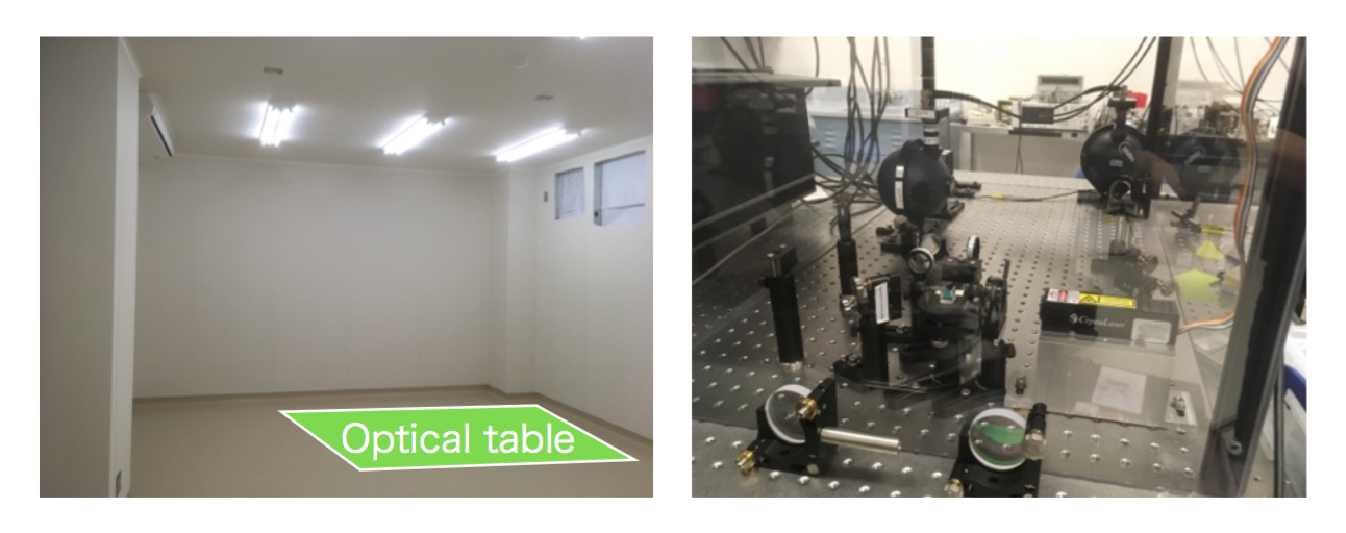
\includegraphics[width=14cm]{Figures/Toyama.eps}
\caption{.} 
\label{fig:Toyama} 
\end{center}
\end{figure}

\begin{figure}
\begin{center}
\includegraphics[width=14cm]{Figures/KWS.eps}
\caption{.} 
\label{fig:KWS} 
\end{center}
\end{figure}

\begin{figure}
\begin{center}
\includegraphics[width=14cm]{Figures/Keithlay.eps}
\caption{.} 
\label{fig:Keithlay} 
\end{center}
\end{figure}
